\noindent Rečová technológia tvorí základ na vytvorenie rozhrania, ktoré umožňuje používateľovi komunikovať so zariadeniami prostredníctvom hovoreného jazyka jednoduchšie než napríklad pomocou grafického displeja, klávesnice alebo myši. Dnes sa takéto hlasové používateľské rozhrania používajú na plne alebo čiastočne automatizované ponuky služieb poskytované spoločnosťami ich zákazníkom, zamestnancom alebo partnerom na telefóne. Obchodné činnosti, ktoré vo veľkej miere závisia od hlasových používateľských rozhraní, sú bankovníctvo, logistika, verejná doprava a~telekomunikácie. Iné využitia technológie rečovej interakcie sú rozhrania pre špeciálne zariadenia, napríklad navigačné systémy do  áut či~uplatnenie hovoreného jazyka ako alternatívy k~vstupno-výstupným modalitám grafických používateľských rozhraní, napríklad v~smartphonoch alebo tabletoch. 

\begin{figure*}[htb]
  \colorrule{grey3}{\textwidth}{1.5pt}
  \center
  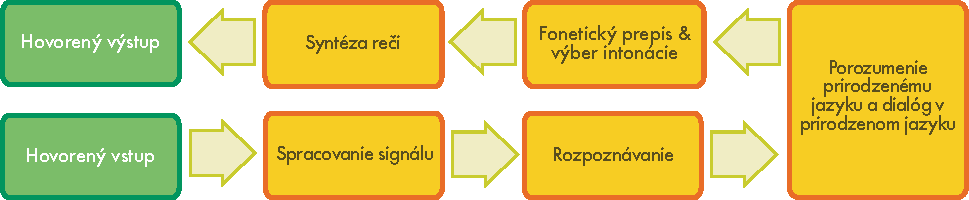
\includegraphics[width=\textwidth]{../_media/slovak/simple_speech-based_dialogue_architecture}
  \caption{Architektúra jednoduchého dialógového systému}
  \label{fig:dialoguearch_sk}
  \colorrule{grey3}{\textwidth}{1.5pt}
\end{figure*}

Vo svojej podstate pozostáva rečová interakcia zo štyroch rôznych technológií:

\begin{itemize}
\item Automatické rozpoznávanie reči zodpovedá za určenie, ktoré slová v~slede zvukov vypovedaných používateľom boli aktuálne hovorené.
\item Syntaktická analýza a~sémantická interpretácia sa zaoberajú analyzovaním syntaktickej štruktúry výpovede používateľa a~jej interpretáciou podľa účelu príslušného systému.
\item Dialógový manažment je potrebný pri určovaní opatrení, ktoré by sa mali podniknúť na strane systému, s~ktorým používateľ komunikuje, vzhľadom na vstup používateľa a~funkčnosť systému.
\item Rečová syntéza (Text-to-Speech, TTS) sa uplatňuje na transformovanie textovej výpovede do zvukovej formy, ktorá bude pre používateľa výstupom.
\end{itemize}

Jednou z~najväčších výziev je vytvoriť systém automatického
rozpoznávania reči, ktorý by dokázal čo najpresnejšie rozpoznať
používateľove slová. To si vyžaduje buď obmedzenie možných
výpovedí používateľa na limitovaný súbor kľúčových slov,
alebo manuálne vytvorenie jazykových modelov, ktoré by pokrývali
veľké množstvo prirodzených výpovedí v~jazyku používateľa.
Základnou požiadavkou pre dobrý výkon je takisto dobre natrénovaný
akustický model založený na obrovskom množstve zaznamenaných dát
rozlišujúcich prízvuk, vekovú skupinu, pohlavie atď. Kým prvá
možnosť vedie skôr k~strnulému a~nepružnému využívaniu
hlasového používateľského rozhrania a~pravdepodobne by ju
používatelia dobre neprijali, tvorenie, ladenie a~zlepšovanie
akustických a~jazykových modelov by zas výrazne zvýšilo náklady.
Hlasové používateľské rozhrania, ktoré využívajú jazykové
modely a dovoľujú na začiatku používateľovi flexibilne vyjadriť
svoju potrebu -- po vyzvaní napríklad frázou „Ako vám môžem
pomôcť“ -- vykazujú lepšiu možnosť automatizácie,
aj~lepšiu akceptáciu používateľmi, a teda majú výhodu oproti
než menej flexibilnému prístupu riadeného dialógu. Výnimku tvoria
tzv. embedded systémy,~ktoré vyžadujú na ovládanie relatívne málo
príkazov. V~takom prípade je použitie jazykových modelov
skôr nevýhodou a~aj dnes sa takéto systémy úspešne budujú
s~použitím gramatík.

Pre výstupné časti hlasového používateľského rozhrania inklinujú spoločnosti k~používaniu vopred nahraných výpovedí profesionálov – ideálne registrovaných hovoriacich. V~prípade statických výpovedí, ktorých obsah nezávisí od kontextu použitia alebo od osobných údajov daného používateľa, bude výsledkom vysoká spokojnosť používateľa. Čím dynamickejší bude obsah výpovede, tým väčšie problémy môže mať používateľ s~nejasnou prozódiou vyplývajúcou z~reťazenia jednotlivých zvukových segmentov. Dnešné systémy na syntézu reči sa vzhľadom na optimalizovateľnú prozodickú prirodzenosť dynamických výpovedí javia ako lepšie. 

Trh technológií rečovej interakcie prešiel počas poslednej dekády silnou štandardizáciou rozhraní medzi odlišnými technologickými komponentmi, ako aj štandardmi na tvorenie daných softvérových artefaktov pre danú aplikáciu. Za posledných desať rokov takisto prebieha silná konsolidácia trhu, hlavne v~oblasti automatického rozpoznávania reči a~syntézy reči. Národné trhy krajín G20, tzn.~ekonomicky silných krajín so značnou populáciou, sú celosvetovo ovládané niekoľkými veľkými súpermi, pričom Nuance, Google a~Microsoft patria dnes medzi najvýznamnejšie.

Na Slovensku má rozpoznávanie reči dlhú históriu, ale vykonávalo sa len na pôde univerzít a~vo vedeckých inštitúciách. Väčšina z~nich sa sústreďuje na základný výskum a~riešenia špecifických problémov rozpoznávania reči. Oddelenie analýzy a~syntézy reči Ústavu informatiky Slovenskej akadémie vied ako účastník projektu SpeechDat-E sa sústreďuje prevažne na akustické modely telefónnych systémov. S~rastúcim množstvom iných rečových nahrávok, ako napríklad parlamentné diskusie, sa ústav pomocou existujúcich nástrojov na rozpoznávanie reči snaží vytvoriť širšie použiteľné akustické modely pre  prepis diktovaného textu. Hlavný dôraz sa kladie na rozpoznávanie reči závislé od rečníka. Katedra elektroniky a~multimediálnych komunikácií Slovenskej Technickej univerzity v Bratislave sa sústreďuje hlavne na spracovanie rečového signálu v~podmienkach hluku (detekcia reči/hluku, extrahovanie atď.). Okrem mnohého iného vytvorila katedra aj početné malé systémy na rozpoznávanie reči, aby mohla porovnávať ich výkonnosť a~použiteľnosť na rozpoznávanie voľnej reči v~slovenskom jazyku. Na~Technickej univerzite v~Košiciach existujú viaceré katedry, ktoré sa sústreďujú na automatické rozpoznávanie reči. Katedra telekomunikácií Slovenskej technickej univerzity sa pôvodne zameriavala na základný výskum digitálneho spracovania rečového signálu, ktorý postupne svoj výskum zamerala na rozvoj rečových interaktívnych systémov.
\newline Katedra vytvorila v~spolupráci so Slovenskou akadémiou vied, Slovenskou technickou univerzitou a~Žilinskou univerzitou inteligentný komunikačný rečový systém, ktorý je prístupný verejnosti v~slovenskom jazyku a~demonštruje rečové interaktívne systémy pri telefonovaní. V~súčasnosti je na katedre jedným z~jej najpozoruhodnejších produktov v~oblasti jazykového modelovania systém na rozpoznávanie plynulej reči. Bázou jazykového modelu  je korpus pozostávajúci z~$2\cdot 10^9$ tokenov. 
\newline Druhé významné pracovné miesto na Technickej univerzite v~Košiciach je Katedra kybernetiky a~umelej inteligencie, kde bol pre slovenčinu vytvorený prvý rečový dialógový informačný systém a~fonetická abeceda SAMPA. Dnes na katedre zohrávajú aktivity týkajúce sa rozpoznávania reči okrajovú rolu. Katedra aplikovanej matematiky a~štatistiky na Fakulte matematiky, fyziky a~informatiky Univerzity Komenského v~Bratislave pracuje predovšetkým na rozpoznávaní reči prostredníctvom izolovaných slov detských hlasov. Výsledky boli aplikované vo vzdelávacom procese na verifikovanie textu čítaného deťmi. Zo zvukových dát zaznamenaných pre akustický modelový nácvik boli vytvorené len dve rečové databázy (\emph{Alica} a~\emph{Viktória}).  Hlavná inštitúcia na rozpoznávanie reči na Žilinskej univerzite je Katedra telekomunikácií a~multimédií. Jej tím sa zameriava predovšetkým na spracovanie digitálneho signálu pre rozpoznanie reči a~rozpoznávanie izolovaných slov pomocou použitia skrytých Markovovských modelov.

Úzka spolupráca medzi Katedrou elektroniky a~multimediálnych komunikácií TU v~Košiciach a~Oddelením analýzy a~syntézy reči Ústavu informatiky Slovenskej akadémie vied vyústila do prvých viditeľných úspechov rozvoja systému na rozpoznávanie plynulej reči. Výsledkom spolupráce je automatický systém prepisovania reči, ktorý možno využiť v~oblasti súdnictva.

Z~komerčných systémov na rozpoznávanie slovenského jazyka stojí za pozornosť produkt českej firmy Newton Technologies, ktorý možno považovať za prvý systém prepisovania v~slovenčine, ktorý je nezávislý od rečníka.

Odhliadnuc od súčasného stavu technológie môžeme konštatovať, že v~blízkej budúcnosti nastanú výrazné zmeny, ktoré budú okrem vplyvov telefónu, internetu a~e-mailových spojení podnietené hlavne rozšírením smartphonov ako novej platformy na manažovanie zákazníckych vzťahov. Tento trend ovplyvní aj využívanie technológií rečovej interakcie. Na jednej strane sa dopyt po hlasových používateľských rozhraniach na telefonickej báze postupom času zníži, na druhej strane používanie hovoreného jazyka ako užívateľsky komfortnej vstupnej modality pre smartphony výrazne získa na dôležitosti. Tento trend je podporovaný aj očividným zlepšením kvality rozpoznávania reči nezávisle od hovoriaceho, a~to pre potreby diktovania, ktoré sa už ponúkajú používateľom smartphonov ako centralizované služby. Ak posunieme outsourcing rozpoznávania reči do infraštruktúry aplikácií, využitie základných lingvistických technológií pre špecifické využitie pravdepodobne v~porovnaní so súčasnosťou získa na dôležitosti.  
